
\part{Principes Généraux}

\section{Jeu au tour par tour}

Batailles Fantastiques : Le 9\ieme{} Âge est un jeu au tour par tour. Une partie ordinaire se joue en 6 Tours de Jeu. Un Tour de Jeu se décompose en deux Tours de Joueur. Un joueur a le premier Tour de Joueur, pendant lequel il déplace ses figurines et attaque avec elles. Après cela, l'autre joueur joue son premier Tour de Joueur, ce qui finit le premier Tour de Jeu. Durant le deuxième Tour de Jeu, le premier joueur joue maintenant son deuxième Tour de Joueur, et ainsi de suite, jusqu'à ce que les deux joueurs aient fait six Tours de Joueur, ce qui termine la partie.

\subsection{Tour de Joueur}

Chaque Tour de Joueur se divise en quatre Phases jouées dans l'ordre suivant :

\hspace*{0.3cm}
\begin{tabular}{c|l}
1 & Phase de Mouvement \tabularnewline
2 & Phase de Magie \tabularnewline
3 & Phase de Tir \tabularnewline
4 & Phase de Corps à Corps \tabularnewline
\end{tabular}

\subsection{Joueur Actif et Joueur Réactif}

Le Joueur Actif est le joueur qui est en train de jouer son tour.

Le Joueur Réactif est le joueur qui n'est pas en train de jouer son tour.

\subsection{Effets simultanés}

À chaque fois qu'au moins deux effets sont activés en même temps, et que leur ordre importe, commencez par résoudre tous les effets contrôlés par le Joueur Actif. Chaque joueur décide de l'ordre dans lequel ses propres effets sont résolus. Si une décision est nécessaire, par exemple pour activer ou non une capacité, le Joueur Actif doit déclarer son choix avant le Joueur Réactif. Une fois que les deux joueurs ont déclaré quelles capacités sont activées et dans quel ordre, les effets sont résolus, en commençant par le Joueur Actif. Par exemple, si les deux joueurs ont une capacité qui peut être activée au début de la Phase de Magie, le joueur dont c'est la Phase de Magie doit décider en premier s'il utilise sa capacité ou non. Ensuite, le Joueur Réactif peut choisir s'il utilise la sienne. Enfin, les effets sont résolus, en commençant par la capacité du Joueur Actif.

\newpage
\section{Les dés}

\subsection{Lancer les dés}

Dans Batailles Fantastiques : Le 9\ieme{} Âge, on utilise souvent des dés pour déterminer ce qu'il s'y passe. Le dé le plus utilisé est un dé à six faces, appelé \og D6 \fg{}, dont les valeurs vont de 1 à 6. Un jet de dé est généralement réussi si le résultat est supérieur ou égal à une certaine valeur, par exemple si le dé donne \result{3} ou plus. Cela est indiqué par un \og 3+ \fg{} (ou 2+, 4+, 6+, etc.). Vous devez quelquefois lancer plusieurs de ces dés en même temps. Cela est représenté par un nombre avant le type de dé, comme \og 3D6 \fg{}, qui signifie qu'il faut lancer 3 dés à six faces et additionner leurs résultats. Dans d'autres cas, un jet de dé peut être modifié par addition ou soustraction d'un chiffre, comme \og 1D6+1 \fg{}. Ajoutez ou soustrayez le chiffre indiqué au résultat du dé. Enfin, certains effets permettent de relancer des dés, comme des jets pour blesser ratés, ou des jets de Sauvegarde Invulnérable ayant donné \result{1}. Relancez simplement le ou les dés en question. La relance d'un dé n'est pas considérée comme un modificateur.

\textbf{Un dé relancé ne peut jamais être relancé à nouveau}, peu importe la raison ou la capacité, et le second résultat doit toujours être accepté.

\paragraph{Lancer un D3}

Il est parfois nécessaire de lancer un D3. Il suffit de lancer un D6 et de diviser le résultat par deux, en arrondissant au supérieur, pour un résultat de 1, 2 ou 3. Quand on parle d'un résultat naturel de \result{1} ou \result{6} à propos d'un jet de D3, on fait toujours référence au résultat du D6 avant la division par deux.

\subsection{Le dé de Direction et Directions Aléatoires}

Le Dé de Direction est un dé à six faces spécial dont toutes les faces sont marquées d'une flèche. Quand une règle demande d'un joueur de déterminer une direction aléatoire, lancez le Dé de Direction et utilisez la direction vers laquelle pointe la flèche obtenue.

\paragraph{Remplacer un Dé de Direction par un D6 classique}

Un dé à six faces ordinaire peut faire l'affaire pour remplacer un Dé de Direction. La face avec un seul point (le \result{1}) pointe dans une direction comme une flèche (voir la figure \ref{figure/deviation_dice}). Si un \result{1} ou un \result{6} est obtenu (\result{1} et \result{6} sont des faces opposées sur un dé standard), utilisez plutôt le point central du \result{5} pour indiquer la direction.

\begin{figure}[!htbp]
\centering
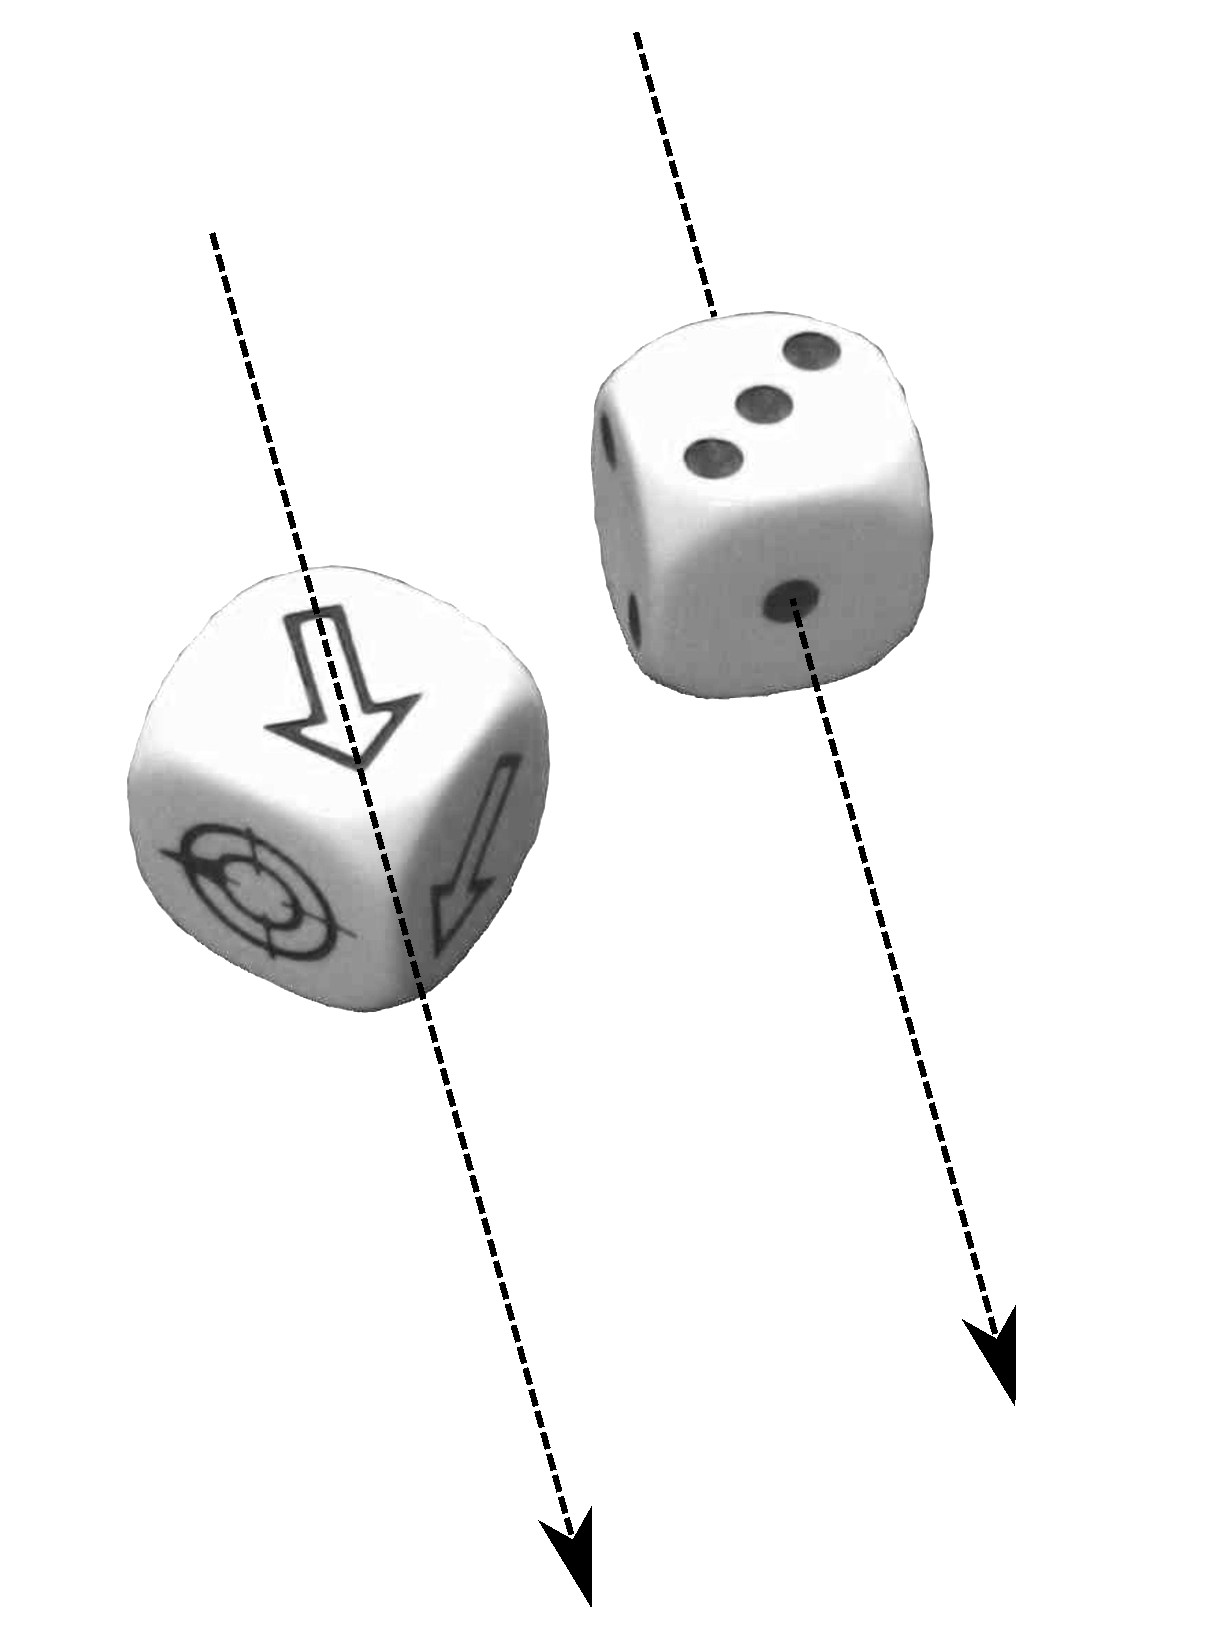
\includegraphics[width=4cm]{pics/deviation_dice.png}
\caption{Deux façons équivalentes de représenter un Dé de Direction.}
\label{figure/deviation_dice}
\end{figure}

